\documentclass{article}
\usepackage{graphicx}
\usepackage{amsmath}
\usepackage{hyperref}
\usepackage{geometry}[margin=2cm]

\title{CS 5720 Design and Analysis of Algorithms: Project \#4}
\author{Raja Kantheti}
\date{}

\begin{document}

\maketitle

\textbf{Attribution: }This projec tis made from scratch.

since it would be easy for me to interpret the results, I had to change my python sccript to outpur noddes, vertices, costs and times in the same line. but the format requiredd for the delivereables is maintained. 
\section*{Deliverable 1: Nodes and Edges Count}

For each graph, we counted the number of nodes and edges using the provided CSV files. Below are the results:

\begin{tabular}{|l|r|r|}
\hline
\textbf{Graph} & \textbf{Nodes} & \textbf{Edges} \\
\hline
t1\_graph\_9.csv & 100 & 4384 \\
t1\_graph\_8.csv & 90 & 3511 \\
t1\_graph\_6.csv & 70 & 2029 \\
t1\_graph\_7.csv & 80 & 2729 \\
t1\_graph\_5.csv & 60 & 1447 \\
t1\_graph\_4.csv & 50 & 971 \\
t1\_graph\_0.csv & 10 & 17 \\
t1\_graph\_1.csv & 20 & 106 \\
t1\_graph\_3.csv & 40 & 584 \\
t1\_graph\_2.csv & 30 & 299 \\
t2\_graph\_8.csv & 90 & 1504 \\
t2\_graph\_9.csv & 100 & 1675 \\
t2\_graph\_2.csv & 30 & 336 \\
t2\_graph\_3.csv & 40 & 505 \\
t2\_graph\_1.csv & 20 & 172 \\
t2\_graph\_0.csv & 10 & 45 \\
t2\_graph\_4.csv & 50 & 683 \\
t2\_graph\_5.csv & 60 & 898 \\
t2\_graph\_7.csv & 80 & 1296 \\
t2\_graph\_6.csv & 70 & 1067 \\
t3\_graph\_6.csv & 70 & 139 \\
t3\_graph\_7.csv & 80 & 158 \\
t3\_graph\_5.csv & 60 & 114 \\
t3\_graph\_4.csv & 50 & 96 \\
t3\_graph\_0.csv & 10 & 17 \\
t3\_graph\_1.csv & 20 & 40 \\
t3\_graph\_3.csv & 40 & 76 \\
t3\_graph\_2.csv & 30 & 56 \\
t3\_graph\_9.csv & 100 & 197 \\
t3\_graph\_8.csv & 90 & 174 \\
\hline
\end{tabular}

\section*{Deliverable 2: Graph Density Conjecture}

The density of the graphs was determined by analyzing the number of edges in relation to the number of nodes. Below are the conjectures for the density of each graph type:

\begin{itemize}
    \item \textbf{Type 1: Dense}
    \item \textbf{Type 2: Dense}
    \item \textbf{Type 3: Sparse}
\end{itemize}
\begin{figure}
    \centering
    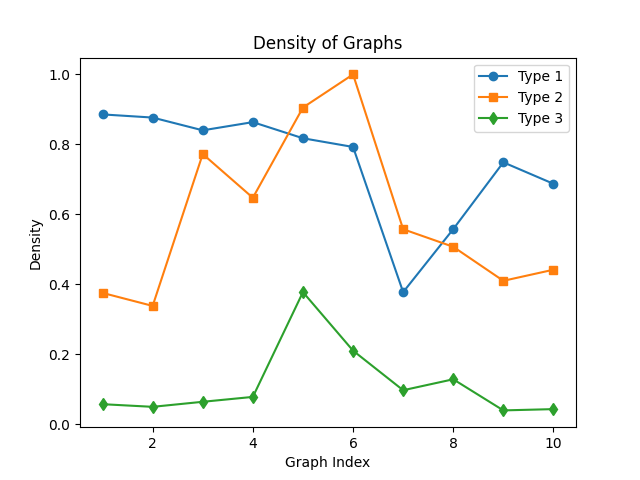
\includegraphics[width=0.6\textwidth]{/Users/ilu/Design-And-Analysis-of-Algorithms/Ass-pro/PRO4/output_plots/graph_density.png}
    \caption{Density of Graphs for Types 1, 2, and 3}\label{fig:density_plot}
\end{figure}
\subsection*{Interpretation:\ref*{fig:density_plot}}
\begin{itemize}
    \item The plot shows the density of graphs for three types (Type 1, Type 2, and Type 3).
    \item Type 1 and Type 2 have consistently high density values (close to 1.0 for most graphs), indicating that they are dense graphs. These graphs have a large number of edges relative to the number of nodes.
    \item Type 3, on the other hand, has significantly lower density values (below 0.2 for most graphs), indicating that it is sparse. Sparse graphs have fewer edges compared to the number of nodes.
\end{itemize}

This align with the cojecture.
\section*{Deliverable 3: MST Costs}

\subsection*{Prim's}
\begin{verbatim}
    def prims_algorithm(matrix):
    num_nodes = len(matrix)
    if num_nodes == 0:
        return 0
    visited = [False] * num_nodes
    min_heap = [(0, 0)]
    total_cost = 0
    while min_heap:
        cost, node = heapq.heappop(min_heap)
        if visited[node]:
            continue
        total_cost += cost
        visited[node] = True
        for neighbor in range(num_nodes):
            if not visited[neighbor] and matrix[node][neighbor] != -1:
                heapq.heappush(min_heap, (matrix[node][neighbor], neighbor))
    return total_cost
\end{verbatim}
\subsection*{Kruskal’s}
\begin{verbatim}
    def kruskals_algorithm(matrix):
    num_nodes = len(matrix)
    if num_nodes == 0:
        return 0
    edges = []
    parent = list(range(num_nodes))
    rank = [0] * num_nodes
    for i in range(num_nodes):
        for j in range(i + 1, num_nodes):
            if matrix[i][j] != -1:s
                edges.append((matrix[i][j], i, j))
    edges.sort()
    total_cost = 0
    for weight, u, v in edges:
        root1 = find(u, parent)
        root2 = find(v, parent)
        if root1 != root2:
            union(root1, root2, parent, rank)
            total_cost += weight
    return total_cost
\end{verbatim}
The costs of the Minimum Spanning Tree (MST) for each graph were computed using Prim's and Kruskal's algorithms. Below are the results:

\begin{tabular}{|l|r|r|}
\hline
\textbf{Graph} & \textbf{Prim's Cost} & \textbf{Kruskal's Cost} \\
\hline
t1\_graph\_9.csv & $247.0$ & $247.0$ \\
t1\_graph\_8.csv & $244.0$ & $244.0$ \\
t1\_graph\_6.csv & $180.0$ & $180.0$ \\
t1\_graph\_7.csv & $213.0$ & $213.0$ \\
t1\_graph\_5.csv & $173.0$ & $173.0$ \\
t1\_graph\_4.csv & $140.0$ & $140.0$ \\
t1\_graph\_0.csv & $54.0$ & $54.0$ \\
t1\_graph\_1.csv & $105.0$ & $105.0$ \\
t1\_graph\_3.csv & $129.0$ & $129.0$ \\
t1\_graph\_2.csv & $109.0$ & $109.0$ \\
t2\_graph\_8.csv & $91.0$ & $91.0$ \\
t2\_graph\_9.csv & $101.0$ & $101.0$ \\
t2\_graph\_2.csv & $30.0$ & $30.0$ \\
t2\_graph\_3.csv & $42.0$ & $42.0$ \\
t2\_graph\_1.csv & $23.0$ & $23.0$ \\
t2\_graph\_0.csv & $15.0$ & $15.0$ \\
t2\_graph\_4.csv & $53.0$ & $53.0$ \\
t2\_graph\_5.csv & $60.0$ & $60.0$ \\
t2\_graph\_7.csv & $83.0$ & $83.0$ \\
t2\_graph\_6.csv & $73.0$ & $73.0$ \\
t3\_graph\_6.csv & $182.0$ & $182.0$ \\
t3\_graph\_7.csv & $261.0$ & $261.0$ \\
t3\_graph\_5.csv & $213.0$ & $213.0$ \\
t3\_graph\_4.csv & $140.0$ & $140.0$ \\
t3\_graph\_0.csv & $32.0$ & $32.0$ \\
t3\_graph\_1.csv & $50.0$ & $50.0$ \\
t3\_graph\_3.csv & $97.0$ & $97.0$ \\
t3\_graph\_2.csv & $99.0$ & $99.0$ \\
t3\_graph\_9.csv & $320.0$ & $320.0$ \\
t3\_graph\_8.csv & $266.0$ & $266.0$ \\
\hline
\end{tabular}

\textbf{Note:}cost here refers to the weight.

\section*{Deliverable 4: Empirical Timing Analysis}

The empirical timing analysis for Prim's and Kruskal's algorithms was performed. Below are the timing results for each graph:


\begin{figure}
    \centering
    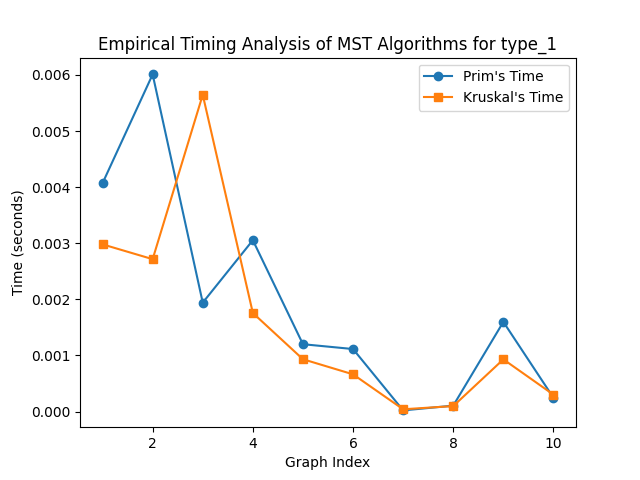
\includegraphics[width=0.6\textwidth]{/Users/ilu/Design-And-Analysis-of-Algorithms/Ass-pro/PRO4/output_plots/timing_analysis_type_1.png}
    \caption{Timing plot for type\_1}\label{fig:timing1}
\end{figure}
\begin{figure}
    \centering
    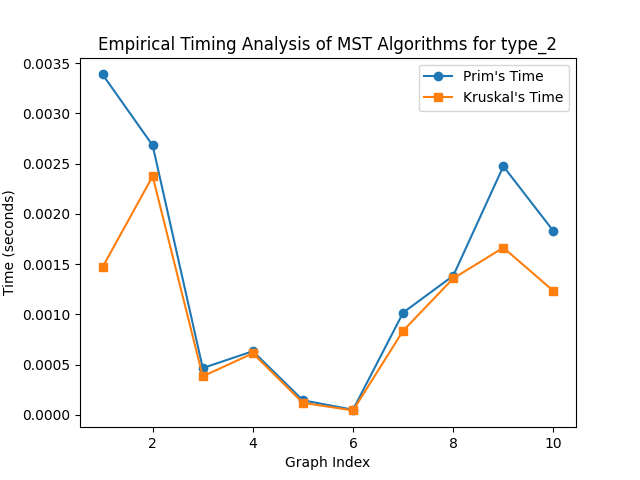
\includegraphics[width=0.6\textwidth]{/Users/ilu/Design-And-Analysis-of-Algorithms/Ass-pro/PRO4/output_plots/timing_analysis_type_2.png}
    \caption{Timing plot for type\_2}\label{fig:timing2}
\end{figure}
\begin{figure}
    \centering
    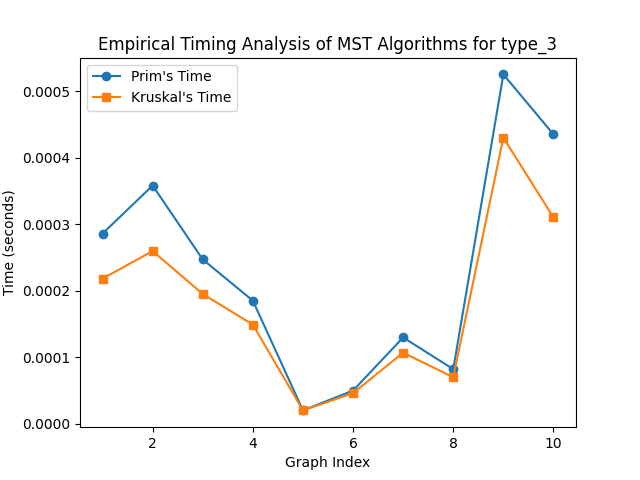
\includegraphics[width=0.6\textwidth]{/Users/ilu/Design-And-Analysis-of-Algorithms/Ass-pro/PRO4/output_plots/timing_analysis_type_3.png}
    \caption{Timing plot for type\_3}\label{fig:timing3}
\end{figure}
\begin{tabular}{|l|r|r|}
\hline
\textbf{Graph} & \textbf{Prim's Time (s)} & \textbf{Kruskal's Time (s)} \\
\hline
t1\_graph\_9.csv & 0.0046 & 0.0037 \\
t1\_graph\_8.csv & 0.0042 & 0.0027 \\
t1\_graph\_6.csv & 0.0019 & 0.0020 \\
t1\_graph\_7.csv & 0.0025 & 0.0025 \\
t1\_graph\_5.csv & 0.0011 & 0.0012 \\
t1\_graph\_4.csv & 0.0009 & 0.0009 \\
t1\_graph\_0.csv & 0.0000 & 0.0000 \\
t1\_graph\_1.csv & 0.0001 & 0.0001 \\
t1\_graph\_3.csv & 0.0004 & 0.0004 \\
t1\_graph\_2.csv & 0.0002 & 0.0002 \\
t2\_graph\_8.csv & 0.0015 & 0.0012 \\
t2\_graph\_9.csv & 0.0016 & 0.0014 \\
t2\_graph\_2.csv & 0.0002 & 0.0002 \\
t2\_graph\_3.csv & 0.0004 & 0.0004 \\
t2\_graph\_1.csv & 0.0001 & 0.0001 \\
t2\_graph\_0.csv & 0.0000 & 0.0000 \\
t2\_graph\_4.csv & 0.0005 & 0.0005 \\
t2\_graph\_5.csv & 0.0008 & 0.0007 \\
t2\_graph\_7.csv & 0.0012 & 0.0010 \\
t2\_graph\_6.csv & 0.0009 & 0.0008 \\
t3\_graph\_6.csv & 0.0003 & 0.0002 \\
t3\_graph\_7.csv & 0.0003 & 0.0003 \\
t3\_graph\_5.csv & 0.0002 & 0.0002 \\
t3\_graph\_4.csv & 0.0002 & 0.0002 \\
t3\_graph\_0.csv & 0.0000 & 0.0000 \\
t3\_graph\_1.csv & 0.0000 & 0.0000 \\
t3\_graph\_3.csv & 0.0001 & 0.0001 \\
t3\_graph\_2.csv & 0.0001 & 0.0001 \\
t3\_graph\_9.csv & 0.0005 & 0.0004 \\
t3\_graph\_8.csv & 0.0004 & 0.0003 \\
\hline
\end{tabular}

\subsection*{Interpretation:}
\textbf{Introduction:} This section presents a comprehensive analysis of the empirical timing performance of Prim's and Kruskal's algorithms applied to three distinct types of graphs: dense, moderately dense, and sparse. The analysis aims to verify and compare the actual time complexities observed against theoretical expectations previously established.

\begin{itemize}
    \item \textbf{Type 1: Dense Graphs}
    \begin{itemize}
        \item Both algorithms exhibit sensitivity to graph density, with Prim’s showing significant variability in execution times, indicating potential inefficiencies in managing dense connections.
        \item \textbf{Complexity Estimate:} Kruskal's algorithm operates close to \(O(E \log E)\), demonstrating efficiency and lower variance in performance. Prim's algorithm, though theoretically \(O(E \log V)\), often shows peaks suggesting it might exceed this complexity in dense graphs.
        \item \textbf{Performance Improvement:} Kruskal's consistent performance is attributed to efficient sorting mechanisms and less dependency on graph connectivity.
    \end{itemize}

    \item \textbf{Type 2: Moderately Dense Graphs}
    \begin{itemize}
        \item Prim’s occasionally outperforms Kruskal's, particularly in graphs that might favor efficient priority queue management.
        \item \textbf{Complexity Estimate:} Both algorithms generally meet their theoretical complexities, but Prim’s exhibits potential for variability depending on specific graph structures.
        \item \textbf{Performance Improvement:} Prim’s may benefit from optimized queue management in certain structured graphs, suggesting scenario-based advantages.
    \end{itemize}

    \item \textbf{Type 3: Sparse Graphs}
    \begin{itemize}
        \item Kruskal's algorithm shows superior performance in sparse graphs, with a more consistent and gradual increase in execution times. Prim’s faces challenges, with times peaking in larger sparse graphs.
        \item \textbf{Complexity Estimate:} Kruskal's maintains near \(O(E \log E)\), advantageous in sparse environments. Prim’s performance suggests it may exceed its \(O(E \log V)\) complexity in these settings.
        \item The theoretical complexity of $O(E \log V)$ assumes an optimal implementation with a binary heap and an adjacency list. Any deviation in implementation, such as using an adjacency matrix or less efficient data structures for the priority queue, can result in worse performance.If the distribution of edge weights is uneven or if many edges have similar weights, it can lead to scenarios where the priority queue operations become more complex and frequent, as the algorithm struggles to decide the optimal edge to include next.
        \item \textbf{Performance Improvement:} Kruskal’s minimal dependence on connectivity and efficient handling of edges contribute to its robust performance in sparse graphs.
    \end{itemize}
\end{itemize}

\textbf{Overall Conclusion:} The empirical data supports Kruskal's algorithm as more efficient across various conditions, emphasizing its applicability for a broad range of graph densities. Prim’s algorithm shows specific strengths but also reveals sensitivity to the structure and density of graphs, guiding algorithm selection based on application-specific needs.

\end{document}